\documentclass[conference,letterpaper]{IEEEtran}
\usepackage[T1]{fontenc}
\usepackage{cite}
\usepackage{amsmath,amssymb}
\usepackage{graphicx,booktabs,array,tabularx}
\usepackage{tikz}
\usetikzlibrary{arrows.meta,positioning,fit,calc}
\usepackage{url}
\usepackage[hidelinks]{hyperref}
\hypersetup{pdftitle={LocalMind: A Local-First Agentic Knowledge Copilot With Persistent Project Memory and a Custom MCP Server},pdfauthor={Trijal Burman; Tiya Singh; Gayatri Rajesh Apotikar; Nimita Jestin},pdfsubject={IEEE-format research manuscript and reproducible synthetic evaluation},pdfkeywords={local-first AI, RAG, MCP, persistent memory, on-device inference}}
\urlstyle{same}
\newcommand{\code}[1]{\texttt{#1}}
\newcommand{\method}{LocalMind}
\hyphenation{data-base data-bases inter-oper-ability}

\begin{document}
\title{LocalMind: A Local-First Agentic Knowledge Copilot With Persistent Project Memory and a Custom MCP Server}
\author{\IEEEauthorblockN{Trijal Burman, Tiya Singh, Gayatri Rajesh Apotikar, and Nimita Jestin}
\IEEEauthorblockA{Symbiosis Institute of Technology}}
\maketitle

\begin{abstract}
Persistent project context is difficult to recover across scattered local documents and conversations without transmitting personal knowledge to hosted services. This paper presents LocalMind, an implemented copilot combining local inference, hybrid retrieval, relational project memory, and a custom Model Context Protocol (MCP) server. A bounded agent reads approved-folder evidence through actual MCP subprocess sessions; SQLite retains extracted text, vectors, notes, and conversations. Frozen experiments use Qwen3 4B and EmbeddingGemma on an RTX 5050 laptop with 16 GB nominal RAM. On the reproducible 39-document LM-Synth v1 corpus, lexical and hybrid retrieval cover all 96 answerable questions within five results. The original generator nevertheless matches 0/24 complete answers because context clipping discards evidence. A subsequent serialized-cost repair retains initial references in 64/64 replayed requests, respects the input budget, and yields 7/24 single-pass and 3/24 agent all-fact value matches without request errors. These inspected-question replays are not held-out confirmation; their passage prefixes still lose facts. Historical summaries visit every section yet retain only 10/24 requested values and have not been rerun. Later development adds exact catalog lookup, query-centered whole-record evidence, model-free greeting routes, and bounded citation retry with extractive fallback. Current verification passes 163 Linux tests and 200 Windows-copy tests on Linux, with six native checks skipped. A separately labeled small 9B development probe does not replace the frozen experiments. Citation checks establish reference integrity, not entailment. No paid inference API is used; general semantic accuracy, adversarial security, and Windows laptop GPU performance remain unverified.
\end{abstract}

\begin{IEEEkeywords}
local-first AI, retrieval-augmented generation, Model Context Protocol, persistent memory, on-device inference, knowledge management
\end{IEEEkeywords}

\section{Introduction}
Knowledge work produces heterogeneous evidence: project notes, source files, reports, decisions, and conversational explanations. Relevant information is often available on a user's disk but absent from the current assistant context. Repeatedly uploading or describing that information increases effort, while hosted inference introduces a separate data-processing boundary. Keeping a long conversation open does not provide a durable, searchable project memory, and increasing a model's context window does not ensure that every relevant fact is used.

Local-first software emphasizes ownership and offline availability \cite{localfirst}. Retrieval-augmented generation (RAG) makes external evidence available to a generator \cite{rag}, while persistent-memory research explores continuity beyond one context window \cite{memgpt,memorybank}. These established directions motivate a practical question: can a modest laptop combine document retrieval, explicit project memory, and interoperable tool use in one locally operated system with inspectable evidence?

We address that question through \method, an implemented web application backed by a local database and local models. A custom MCP server separates knowledge access from the conversational host \cite{mcp}. The application allows a user to approve folders on an HDD or SSD, index supported text, inspect complete extracted contents, ask grounded questions, save memories, and draft project plans. It does not automatically scan every drive or execute generated software. Initial installation requires downloads; subsequent document processing and inference can operate without a hosted API.

This paper makes three contributions. First, it describes the concrete integration of local inference, hybrid retrieval, relational project memory, and actual MCP subprocess communication, including the controls that bound the agent's capabilities. Second, it distinguishes complete extraction, retrieved evidence, reference integrity, and generated factual coverage. Third, it supplies a frozen synthetic corpus, executable evaluation, raw outputs, and laptop measurements, with separately labeled production-repair and later development checks. These checks leave the original results unchanged. None of RAG, rank fusion, memory, or MCP is proposed as a new algorithm.

Four research questions structure the evaluation: \emph{RQ1}, how do lexical, dense, and fused retrieval cover labeled evidence? \emph{RQ2}, how does the bounded MCP agent compare with single-pass local RAG on answer-value matching and missing information? \emph{RQ3}, does processing every extracted section retain the requested facts in the final summary? \emph{RQ4}, what runtime costs and functional guarantees are supported on the measured platforms? The answers are conditional on the stated corpus, implementation revisions, and hardware.

\section{Related Work}
\subsection{Retrieval and Grounded Generation}
RAG combines retrieved nonparametric knowledge with generation \cite{rag}. Dense Passage Retrieval uses learned dual encoders for passage matching \cite{dpr}; Sentence-BERT demonstrates efficient independent representations for similarity computations \cite{sbert}. BM25 remains a strong lexical foundation with term-frequency saturation and length normalization \cite{bm25}. Dense representations can help with paraphrases, while lexical retrieval preserves identifiers and exact terminology. Their relative value depends on the corpus and query distribution.

Reciprocal rank fusion (RRF) combines ranked lists without requiring their raw scores to share a scale \cite{rrf}. \method\ applies this established technique to SQLite FTS5 and local cosine retrieval. It does not train the retriever jointly with the generator, fine-tune embeddings, or implement an approximate nearest-neighbor index. Accordingly, the present comparison concerns the deployed pipeline rather than the performance of the original RAG or DPR systems.

\subsection{Tool Use and Persistent Memory}
ReAct interleaves information gathering with model-selected actions \cite{react}. Toolformer studies learning when and how to invoke APIs \cite{toolformer}. \method\ uses an already trained model and a bounded runtime loop; it neither reproduces Toolformer's training procedure nor exposes internal reasoning as an experimental variable.

MemGPT investigates hierarchical memory and virtual context management \cite{memgpt}. MemoryBank targets persistent user-oriented memory \cite{memorybank}, and LongMem incorporates a learned memory architecture \cite{longmem}. Generative Agents uses memory and reflection for simulated behavior \cite{genagents}; Reflexion studies feedback retained across trials \cite{reflexion}. In contrast, \method\ stores explicit notes, projects, and conversations in ordinary relational records. It has no learned memory consolidation, forgetting policy, autonomous reflection, or automatic preference extraction. Explicit user control over writes is a deliberate capability restriction.

\subsection{Context, Ownership, and Interoperability}
Long contexts do not remove selection and position effects: Lost in the Middle reports that relevant information can be used unevenly across input positions \cite{lostmiddle}. This motivates separating evidence retrieval from full-document processing and measuring the latter's retained facts. A section trace establishes that text entered a processing stage; it cannot establish semantic completeness.

The broader local-first vision includes collaboration and replication \cite{localfirst}. \method\ implements single-laptop ownership and offline operation, not collaborative synchronization or conflict-free replicated data types. MCP supplies a common host--client--server interface for tools and resources \cite{mcp}; interoperability does not itself enforce authorization. Indirect prompt injection further motivates treating retrieved content as untrusted \cite{injection}. Local inference changes where processing occurs, while runtime capabilities determine what a compromised response can do.

\subsection{Evaluation Foundations}
BEIR emphasizes heterogeneous retrieval evaluation and the importance of lexical baselines \cite{beir}; MTEB evaluates embeddings across tasks \cite{mteb}. RAGAs separates retrieval, faithfulness, and answer quality \cite{ragas}, while citation-oriented generation research evaluates whether references support claims \cite{alce}. We retain those distinctions. Public model scores are not transferred to this implementation, and quantitative scores use no model judge. LM-Synth supports transparent value-level diagnostics, with a narrower scope than those public benchmarks.

\section{Requirements and Threat Model}
The target deployment is one trusted user on a laptop with a Ryzen 7 250, RTX 5050, and 16 GB nominal RAM. The design requires persistent project context, source-backed answers, complete extracted-text access, bounded inference, and continued lexical operation when models are unavailable. The system must not require a paid API, hosted vector service, or remote database. ``No paid inference API'' does not mean zero hardware, electricity, storage, bandwidth, or maintenance cost.

The privacy boundary contains the local browser, API, SQLite database, approved document folders, MCP subprocess, and loopback model server. Application inference endpoints accept HTTP loopback hosts only, reject remote-model metadata, and bypass inherited HTTP proxies. Bundled UI assets avoid a CDN dependency. The model runtime is configured with cloud access disabled \cite{ollama}. These controls describe application data flow; they are not a formal proof that the operating system or all installed software is offline.

We consider accidental overbroad folder selection, stale documents, indirect instructions in retrieved text, malformed tool arguments, and unbounded tool execution. We do not assume resistance to a compromised OS account, malicious kernel, physical disk access, or a hostile application with the same file permissions. SQLite is not encrypted by the application. Known-secret filename exclusions are heuristics; an ordinary note can still contain sensitive information. A hosted external MCP client can transmit returned data outside this boundary.

The Linux scanner rejects protected system roots and symbolic-link traversal, but it does not identify the physical backing type of every mounted filesystem. An explicitly approved network-backed mount is therefore outside a strict physical-local-disk guarantee. The Windows edition additionally restricts accepted paths to supported local fixed/removable drives and rejects UNC/network paths, junctions, and reparse-backed sources. This platform difference is preserved rather than concealed by a universal privacy claim.

\section{System Architecture}
\begin{figure*}[t]
\centering
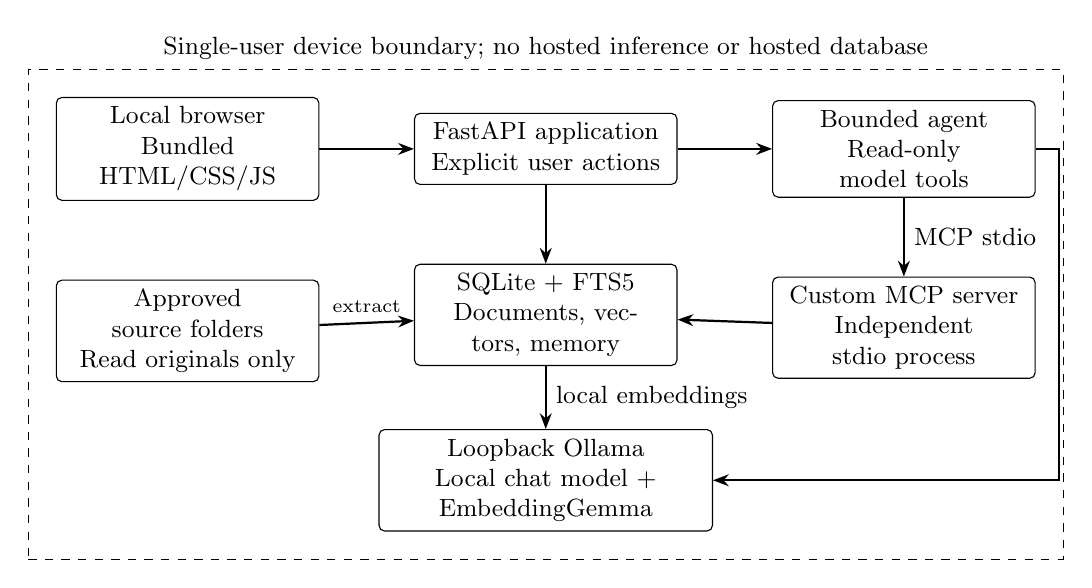
\begin{tikzpicture}[font=\small,box/.style={draw,rounded corners=2pt,align=center,minimum height=0.85cm,text width=3.1cm},arr/.style={-{Stealth[length=2mm]},thick},node distance=0.7cm and 1.2cm]
\node[box] (ui) {Local browser\\Bundled HTML/CSS/JS};
\node[box,right=of ui] (api) {FastAPI application\\Explicit user actions};
\node[box,right=of api] (agent) {Bounded agent\\Read-only model tools};
\node[box,below=1.0cm of ui] (files) {Approved source folders\\Read originals only};
\node[box,below=1.0cm of api] (db) {SQLite + FTS5\\Documents, vectors, memory};
\node[box,below=1.0cm of agent] (mcp) {Custom MCP server\\Independent stdio process};
\node[box,below=0.8cm of db,text width=4cm] (llm) {Loopback Ollama\\Local chat model + EmbeddingGemma};
\draw[arr] (ui) -- (api);
\draw[arr] (api) -- (agent);
\draw[arr] (files) -- node[above,font=\scriptsize]{extract} (db);
\draw[arr] (api) -- (db);
\draw[arr] (agent) -- node[right]{MCP stdio} (mcp);
\draw[arr] (mcp) -- (db);
\draw[arr] (agent.east) -- ++(0.3,0) |- (llm.east);
\draw[arr] (db) -- node[right]{local embeddings} (llm);
\node[draw,dashed,fit=(ui)(api)(agent)(files)(db)(mcp)(llm),inner sep=0.35cm,label={[font=\small]above:Single-user device boundary; no hosted inference or hosted database}] {};
\end{tikzpicture}
\caption{Implemented data flow. Original files are read through approved roots. The API and MCP server share relational storage. The model receives bounded evidence through the agent; it receives no source-file write or shell tool. The boundary assumes trusted local software and a locally operated MCP client.}
\label{fig:architecture}
\end{figure*}

\subsection{Components and Persistent State}
Fig.~\ref{fig:architecture} shows the deployed components. A bundled browser UI communicates with FastAPI, which coordinates indexing, conversations, memories, and projects. Ollama provides the chat model and text embeddings over loopback. The official Python MCP SDK launches and negotiates the separate memory service; the protocol boundary is exercised by actual subprocess tests, not simulated function names \cite{localmind}.

SQLite stores approved roots, document metadata and full extracted text, offset-preserving chunks, vector BLOBs, explicit memories, projects, sessions, and messages. FTS5 indexes chunk content and conversation messages \cite{sqlite}. Short-lived connections, foreign keys, a busy timeout, and write-ahead logging support normal reads while another process writes. The API and MCP client share the same configured data directory.

Explicit memory is a relational note with a kind and optional project identifier. Memory lookup uses bounded substring filtering; conversation lookup uses FTS5. Neither is a knowledge graph or a semantic vector index over every past chat. The agent initially selects bounded global and project notes, while project filtering limits relevant conversation tools. Persistence and retrieval are separate: saving a note does not guarantee that it will fit every future prompt.

\subsection{Approved Ingestion and Complete Text}
The user selects existing folders; the app rejects overlapping roots, its own data directory, protected roots, and unsupported links. Scanning skips hidden items, known credential names, dependencies, and unsupported formats. Text and common code files are decoded locally. PDF text is extracted with page boundaries, and DOCX text is extracted from relevant XML parts, including tables and available notes. No OCR, image interpretation, or visual-layout reproduction is provided.

Table~\ref{tab:limits} lists implemented bounds. Opening each Linux path component without following links helps prevent replacement through a symbolic link. Windows uses native handles and reparse-point checks. Extracted text is stored in full as a snapshot, with exact character offsets in each chunk. PDF chunks stay within a page. ``Complete contents'' therefore means the complete successful text extraction of a supported indexed file, not the original formatting or every byte on a drive.

\begin{table}[t]
\caption{Implemented Resource and Execution Bounds}
\label{tab:limits}
\centering\small
\begin{tabularx}{\columnwidth}{@{}lX@{}}
\toprule
Parameter & Bound or default \\
\midrule
Original source size & 20 MiB per file \\
Scan candidates & 20,000 supported files \\
Extracted text / PDF & 5,000,000 characters / 2,000 pages \\
Chunk / overlap & 1,800 / 200 characters \\
Embedding batch & 16 chunk texts \\
Stored vector & Float32 BLOB, model tag, dimension \\
MCP document page & Up to 50,000 characters \\
Chat context & 8,192 tokens by default; optional local profile 12,288 \\
Agent loop & 4 model/tool rounds; at most 6 additional tool executions \\
Final synthesis & At most one additional call, tools disabled \\
Citation retry & At most one further call, tools disabled \\
Summary section & Up to 4,000 characters at the default context \\
\bottomrule
\end{tabularx}
\end{table}

Incremental scans compare modification time and size; changed documents replace their extraction and chunks, while unchanged documents can receive missing embeddings. Removed rows are pruned only after complete enumeration. Retrieval and complete-text reads reject sources whose recorded metadata is stale. This is metadata-based freshness, not cryptographic verification: changes preserving both size and timestamp can evade it. Rescans are explicit; there is no background watcher.

\subsection{Model Configuration}
The frozen experiments use Qwen3 4B Instruct 2507 in Q4\_K\_M quantization, tagged \code{qwen3:4b-instruct-2507-q4\_K\_M}, with an 8,192-token chat context. Qwen3's family report provides model background, while the artifact tag and digest identify the actual experiment \cite{qwen}. The embedding artifact is \code{embeddinggemma:latest}, a roughly 308M-parameter BF16 representation model with 768 output dimensions and a 2,048-token input context \cite{gemma}. Its context is independent of the chat setting.

The application uses temperature 0.25, a generation cap of 1,536 tokens at the default context, ten-minute keep-alives, and no hosted fallback. The production seed is not fixed. The frozen experiment retains these settings without selecting outputs from repeated attempts. Setup defaults remain the 4B model and 8,192 tokens. A later optional local profile uses \code{qwen3.5:9b-q4\_K\_M}, 12,288 tokens, and thinking disabled; its small development probe is reported separately. Changing model, context, and integration together does not isolate a model-quality effect. Digests, options, and run identities accompany the respective records.

\section{Retrieval and Memory Access}
\subsection{Chunking and Lexical Ranking}
For document text $x$, a chunk $c_i=x[a_i:b_i]$ preserves exact offsets. Chunking targets 1,800 characters and prefers a newline or sentence delimiter in the latter half of the candidate window; adjacent chunks overlap by 200 characters. These are character limits, not token limits. The overlap reduces boundary losses without making extraction or model input unlimited.

FTS5 searches text, title, and path using BM25 field weights 1.0, 2.0, and 0.3, respectively. The application tokenizes at most 24 distinct query words and joins them with OR. Generic BM25 combines inverse document frequency, saturated term frequency, and length normalization \cite{bm25}; SQLite negates its BM25 score, so lower values rank first \cite{sqlite}. Identifiers and project names can therefore dominate this small corpus, an effect considered when interpreting dense retrieval.

\subsection{Dense Ranking and Fusion}
Let $q\in\mathbb{R}^{768}$ be a query embedding and $v_i$ a compatible stored chunk vector. Dense similarity is
\begin{equation}
s(q,v_i)=\frac{q^\top v_i}{\lVert q\rVert_2\lVert v_i\rVert_2}.
\label{eq:cosine}
\end{equation}
The implementation checks finite, nonzero vectors, compatible dimensions, and matching model labels. Only positive cosine candidates enter the semantic ranking. It scans vectors in batches of 128 rows and retains a bounded heap rather than loading a large Python list of every vector.

For lexical and dense ranks $r_L(c)$ and $r_D(c)$, absent terms contributing zero, fusion is
\begin{equation}
R(c)=\frac{\mathbb{1}[c\in L]}{60+r_L(c)}+
      \frac{\mathbb{1}[c\in D]}{60+r_D(c)}.
\label{eq:rrf}
\end{equation}
The constant 60 follows the established RRF method \cite{rrf}. Candidate depth is $\min(160,\max(40,4\ell))$, where $\ell$ is the store-level requested limit. The library overfetches before checking source freshness. Ties use deterministic chunk identifiers. If embeddings are unavailable or fail, lexical search remains usable.

This is exhaustive cosine retrieval with $O(Nd)$ similarity work per query for $N$ compatible chunks of dimension $d$, plus bounded candidate retention. Streaming bounds working memory for ranking; it does not establish constant memory for extraction, model inference, or the full application. No large-archive scalability result is claimed.

\subsection{MCP Contract and Capability Boundary}
The server exposes knowledge search, paginated document reading, memory recall, project/document listing, conversation search, and explicit memory/project mutations. Tools carry protocol annotations and validated argument bounds. The host negotiates an actual SDK session, discovers schemas, and exchanges structured results over stdio. Stdout is reserved for protocol messages.

The built-in model sees seven read tools: knowledge search, document read, recall, document listing, exact document finding, project listing, and conversation search. The catalog returns bounded pages with a total and next offset; exact lookup distinguishes basenames, absolute paths, and root-relative paths, including duplicate basenames. A negative lookup concerns the indexed catalog, not every file on disk. Linux preserves native case-sensitive identity and Windows uses its platform-specific matching rules. A requested tool outside the allowlist is rejected. Annotations do not enforce authorization. External clients can access server write tools and must impose their own policy. No tool executes a shell or reads an arbitrary caller-supplied filesystem path.

\section{Bounded Agent and Full-Document Processing}
\subsection{Conversation Workflow}
Full-string greeting, thanks, identity, and help patterns return a small model-free response before model readiness checks, MCP startup, history loading, or document retrieval. A greeting combined with a substantive request follows the ordinary workflow. Explicit current-user memory commands such as \code{/remember} write notes directly; retrieved text cannot invoke them. Catalog-listing and exact-filename questions use metadata routes rather than asking a generator to infer the inventory from five search hits.

For ordinary questions, the agent initializes MCP, requests five source passages, and recalls saved context. History, memories, project metadata, and passages are reference data. The system instruction prioritizes the current request, distinguishes evidence from inference, and forbids treating a retrieved project's identity as the user's current project. Exact filenames come from metadata. The assistant can explain documented commands but has no tool to start a server, inspect live sensors, or perform system checks.

The model can request additional read operations over at most four rounds. A per-turn cap permits at most six additional tool executions, excluding the initial search and recall. A final tool-free synthesis call bounds completion. Tool errors are returned as data and recorded in the trace. This is a constrained agentic workflow inspired by tool-using systems \cite{react}, not an unrestricted autonomous agent.

The fitter reserves generation and framing space, pins the system instruction and latest user request, and uses a conservative UTF-8 byte budget rather than exact tokenizer counts. Binary search accounts for actual serialized cost, including JSON escaping and shortening markers. Schemas are counted and may be omitted; tool-call metadata stays whole. The frozen baseline could discard an evidence block after a serialization overshoot. The historical diagnostic and production replay isolate that repair in Section~VIII.

Current evidence preparation adds a separate whole-record check. It selects query-centered contiguous excerpts, initially up to 1,000 characters per source, and reduces windows fairly against the actual fitted payload. Each JSON record retains its complete source number, title, document identifier, and path. If all identities cannot fit, bounded subset selection can skip an oversized record instead of truncating its identity or emitting partial JSON. Visible records are numbered consecutively, and returned cards use exactly the fitted excerpts. After further reads or searches, evidence is repacked from the original source pool. Final synthesis removes tool schemas and repacks again so its cards describe that call's evidence. Bounded windows and omitted records can still lose required facts.

When document sources are present, citation requirements also apply to imperative requests such as ``explain'' or ``summarize''; they do not depend on interrogative wording. Code indices are excluded from citation parsing, and retained conversation evidence has a separate allowance. Explicit invalid reference indices trigger extractive fallback. A response missing required citations receives at most one tool-free regeneration with fresh, complete evidence and a pinned citation instruction. It is checked by the same guard; success uses the retry's cards, while failure keeps the original extractive fallback and its cards. These checks establish reference integrity, not semantic entailment or the truth of capability claims. UI cards group passages by document while preserving their original citation numbers, exact identity, actual nonempty excerpt count, and available PDF pages.

If the chat model is not ready, the app returns a labeled extractive mode with matching excerpts. A document-specific request without a ready model returns a preview and a complete-text reading option, not an alleged AI summary. An installed but failing inference server can still produce a surfaced error; the presence check is not a guarantee of successful generation.

\subsection{Complete-Document Summarization}
A document-specific request follows MCP pagination until the complete extraction is read. The agent divides text into sections of
\begin{equation}
h=\max(150,\min(4000,C-3200))\text{ characters},
\end{equation}
where $C$ is the configured chat context. Each section is summarized, then partial summaries are recursively merged. At the default configuration, $h=4000$; merge input truncates each partial to at most $h/2$ characters, and merge outputs are similarly bounded to ensure convergence.

This process considers every input section but introduces a compression bottleneck. Facts can be omitted during the map stage or truncated during merging. We therefore measure two separate quantities: section-processing coverage and final requested-fact retention. Neither a trace of every section nor a successful full-text transport test establishes perfect summarization. This distinction also addresses context-position concerns raised in prior work \cite{lostmiddle}.

\subsection{Project Planning}
A project stores a name, description, and linked notes. A user-triggered plan retrieves indexed evidence through MCP and asks the local model for goals, milestones, architecture, tasks, acceptance criteria, and next steps. Sources found during retrieval are appended as local references, and the result is saved as the project's \code{PLAN.md}. The implementation drafts a plan; it does not scaffold, compile, or execute arbitrary project code. Appended references improve traceability but do not automatically validate every proposed task or date.

\section{Experimental Method}
\subsection{Versions, Hardware, and Execution}
The frozen baseline uses Linux commit \code{ddbbbb7}, preserved separately from the Windows edition \cite{localmind}. The production replay captured a then-uncommitted repair of \code{copilot/ollama.py}; Appendix~\ref{app:reproduction} records its SHA-256 identity. Later published snapshots are Linux \code{4a3533a} and Windows \code{b377ac6}; subsequent routing checks are later development evidence, not reruns of the frozen experiments. Experiments were executed on 17 October 2026 on a Ryzen 7 250 with eight cores and sixteen threads, an RTX 5050 Laptop GPU reporting 8,151 MiB VRAM, and 16 GB nominal RAM (14,768 MiB visible to the OS). The host ran Linux 7.0.0-38-generic, NVIDIA driver 595.99.02, CPython 3.14.4, and Ollama 0.35.0. Dedicated loopback servers on ports 11437 (historical runs) and 11438 (production replay) reused downloaded models with cloud inference disabled. No personal source folders entered the research corpus.

The Python environment used NumPy 2.5.3, HTTPX 0.28.1, MCP SDK 1.30.0, FastAPI 0.142.2, and pypdf 6.19.0. Warm-up used a non-answer-bearing readiness prompt. Generation temperature remained 0.25 with no fixed seed. Each frozen primary condition was run once per question, without prompt search, model training, answer selection, or retry of unsuccessful outputs. The initial context-fitter adapter was designed after observing the baseline failure. A later production replay exercises the repaired application directly, with actual MCP calls and no fitter substitution. Both reuse the original 24 answerable and eight absent-value items per method; neither is held-out confirmation. Retrieval and summary measurements remain frozen and are not rerun by this generation-only verification.

\subsection{LM-Synth v1 Corpus}
LM-Synth v1 is an authored, deterministic English corpus with seed 20261017. Template and builder-code drafting used AI assistance; the evaluated Qwen3 and EmbeddingGemma models did not generate gold labels or judge outputs. Twelve fictional project families each contain decisions, specifications, and operations records, for 36 ordinary Markdown files. Three additional readiness dossiers support long-document tasks. The corpus has 201,518 Python characters. Ordinary files contain 3,953--4,528 characters; long files contain 16,214, 16,214, and 16,224 characters.

The question set contains 48 lexical, 36 paraphrase, and 12 two-document answerable questions, totaling 96. Each cross-document question requires two gold facts from distinct files; the answerable set therefore contains 108 required fact instances. Eight additional questions request values absent from the sources. Three summary requests each ask for eight facts spread from the beginning to the end of a long dossier. Gold labels specify literal values, permitted rendering aliases, and exact relative document paths. A matching value in the wrong file does not count as retrieved evidence.

Templates and labels were fixed before evaluated-model execution. The dataset, scorer, outputs, and gold-label files remain outside the approved corpus folder; the values themselves occur in the source documents by design. No private documents, real personal conversations, or evaluated-model-generated answers were used to tune the corpus. Repeated project templates and retained project names intentionally make the study easy to audit, but constrain external validity. In particular, a paraphrase question is not a pure test of semantic matching if it still shares a project identifier.

\subsection{Retrieval Conditions and Measures}
All answerable questions are evaluated under three conditions: lexical FTS5, cosine-only dense retrieval, and production-style RRF hybrid retrieval. The same indexed text and local vectors are used. Lexical/hybrid ranking uses candidate lists of up to 60 entries, corresponding to the store-level overfetch used for five final passages, and records the top ten results. The dense-only quality control sorts vectorized cosine scores across all 141 chunks and retains ten; its ranking time is not treated as a comparable production service latency. Documents remain unchanged during this comparison, so freshness rejection is not a relevance confound. Every chunk must have a finite, nonzero, model-compatible 768-dimensional embedding.

For query $q$ with required facts $F_q$, let $G_{qj}$ be the set of correct-document chunks containing an accepted value for fact $j$, and let $T_k(q)$ be the first $k$ results. We measure evidence-fact recall as
\begin{equation}
\operatorname{EFR@}k=\frac{1}{|Q|}\sum_{q\in Q}\frac{1}{|F_q|}
 \sum_{j\in F_q}\mathbb{1}[T_k(q)\cap G_{qj}\ne\varnothing].
\end{equation}
Complete-evidence success (CES@$k$) requires all facts for a question to be covered. MRR@10 uses the first chunk containing any required fact; it does not require both cross-document facts. These definitions prevent duplicated overlapping chunks from inflating fact recall. Their operational evidence labels use accepted value strings and document paths, not independently annotated entailment or semantic relevance. CES@5 intervals use 2,000 bootstrap resamples of the twelve project clusters, preserving dependence among questions within each project.

\subsection{Generation Conditions and Measures}
Generation uses 24 answerable questions, selected by predetermined rotating query-index pairs across projects, giving eight lexical, eight paraphrase, and eight cross-document tasks. All eight absent-value questions are added. The two conditions are single-pass in-process hybrid RAG and the actual bounded MCP agent. They use the same model, context setting, initial five-hit retrieval policy, and a request for at most two sentences. Each asks for the phrase ``Not in the documents'' when the answer is absent. Hash-determined condition order is balanced 12/12 over answerable items; overall it is 19 agent-first and 13 single-pass-first, so full-set timing is not perfectly counterbalanced.

The single-pass condition omits tool schemas and additional tool calls. The agent additionally incurs MCP initialization, recall, schema context, and possible extra model/tool calls. This is an end-to-end method comparison, not an isolated estimate of MCP protocol overhead or a perfectly controlled ablation of action selection. Responses are not stored as conversation messages, and the evaluation asserts that no prior answer or memory row can leak into later questions.

Fact-value match (FVM) checks case-folded, punctuation-insensitive aliases. All-fact value match (AFVM) requires every requested value in an answer; partial FVM averages fact coverage per question. These are transparent string-based proxies, not human judgments of semantic correctness: a negated, misattributed, or contradictory mention can pass. Citation-index validity and coverage of gold document paths are measured separately; they are not citation entailment or claim-level precision. Absence behavior includes the strict requested-phrase rate. AFVM uncertainty is summarized with project-cluster bootstrap intervals; the small missing-value set is reported with its denominator.

\subsection{Summaries, Resources, and Reproducibility}
The three long documents are summarized through the actual document-specific MCP and map/merge path. Each requires five sections at the configured section size. Section traces and final matching gold values are retained separately. Twenty-four requested facts across three templates provide a diagnostic retention measure, not a general summarization benchmark or a test of unsupported-claim rate.

End-to-end times include the operations used by each method. Successful and failed chat attempts, token counters where returned, tool traces, and raw responses are retained. A one-second sampler records total device GPU memory and utilization, plus the summed resident memory of the benchmark process, explicitly selected runtime server, and their descendants. Summed RSS can double-count shared pages; total GPU memory includes the desktop. These observations are neither isolated model allocation nor energy measurements.

Each run stores dataset and corpus-file SHA-256 hashes, model digests, harness hash, options, and package versions. Resume is rejected if identity changes; a new run identifier is required. Failures are retained rather than silently removed. The accompanying builder's \code{--check} option verifies byte-identical synthetic artifacts. These measures support auditability without exposing private files.

\section{Results}
\subsection{Retrieval Effectiveness (RQ1)}
All 39 documents were indexed without an extraction or embedding error, producing 141 chunks. Table~\ref{tab:retrieval} reports complete-evidence success. Lexical and hybrid retrieval both cover all required facts for 96/96 questions within five results; dense retrieval covers 91/96. The five dense failures occur among paraphrase questions, yielding 31/36 in that category. All three methods achieve complete coverage at ten results. This is evidence retrieval on the synthetic questions, not 100\% answer accuracy.

\begin{table}[t]
\caption{Complete-Evidence Success on 96 Answerable Questions}
\label{tab:retrieval}
\centering\small
\begin{tabular}{@{}lrrrr@{}}
\toprule
Method & CES@1 & CES@3 & CES@5 & MRR@10 \\
\midrule
Lexical & 86.46\% & 93.75\% & 100.00\% & 0.9948 \\
Dense & 68.75\% & 91.67\% & 94.79\% & 0.8755 \\
Hybrid RRF & 80.21\% & 94.79\% & 100.00\% & 0.9495 \\
\bottomrule
\end{tabular}
\vspace{3pt}
\parbox{\columnwidth}{\footnotesize CES requires both sources for a two-document question. At five results, project-cluster bootstrap intervals are [100,100]\% for lexical/hybrid and [91.67,97.92]\% for dense. Degenerate empirical intervals do not establish population certainty.}
\end{table}

\begin{figure}[t]
\centering
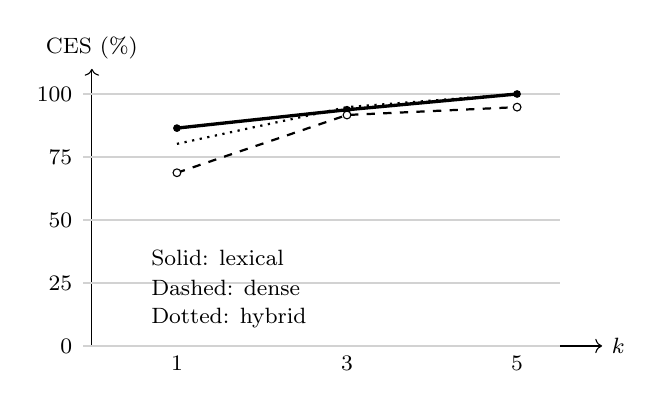
\begin{tikzpicture}[x=1.8cm,y=0.032cm,font=\footnotesize]
\draw[->] (0,0) -- (0,110) node[above,align=center]{CES (\%)};
\draw[->] (0,0) -- (3.6,0) node[right]{$k$};
\foreach \y in {0,25,50,75,100} {\draw[gray!35] (-0.06,\y) -- (3.3,\y);\node[left] at (-0.07,\y){\y};}
\foreach \x/\k in {0.6/1,1.8/3,3.0/5} {\node[below] at (\x,0){\k};}
\draw[very thick] (0.6,86.46) -- (1.8,93.75) -- (3.0,100);
\draw[thick,dashed] (0.6,68.75) -- (1.8,91.67) -- (3.0,94.79);
\draw[thick,dotted] (0.6,80.21) -- (1.8,94.79) -- (3.0,100);
\foreach \x/\y in {0.6/86.46,1.8/93.75,3.0/100}{\fill (\x,\y) circle (1.4pt);}
\foreach \x/\y in {0.6/68.75,1.8/91.67,3.0/94.79}{\draw[fill=white] (\x,\y) circle (1.4pt);}
\node[anchor=west] at (0.35,35){Solid: lexical};
\node[anchor=west] at (0.35,23){Dashed: dense};
\node[anchor=west] at (0.35,11){Dotted: hybrid};
\end{tikzpicture}
\caption{Evidence coverage improves with the result budget. Fusion matches lexical CES@5 but does not improve its first-relevant-hit rank on this identifier-rich synthetic corpus.}
\label{fig:retrieval}
\end{figure}

First-result evidence-fact recall is 92.71\%, 75.00\%, and 86.46\% for lexical, dense, and hybrid, respectively. Hybrid improves coverage over dense at five results, but adds no CES@5 gain over lexical and has lower MRR. The retained project names and repeated document structure favor exact lexical signals. Fig.~\ref{fig:retrieval} therefore supports retaining a lexical baseline rather than presuming that fusion is always superior. No public benchmark performance or general superiority is inferred.

\subsection{Frozen-Baseline Answer Behavior (RQ2)}
The frozen baseline produces a counterintuitive failure: both single-pass RAG and the original MCP agent match zero complete answers out of 24 answerable questions and have zero partial fact-value recall. Both return the requested absence phrase on all eight missing-value questions, but also on all 24 positive questions. No additional model-selected tool executes, no inference request errors, and each response uses one successful chat call. Thus 8/8 absence-phrase compliance is an always-abstain outcome, not evidence of calibrated missing-information handling.

The primary result is retained unchanged. The full retrieved sources cover all 32 required fact slots for the 24 generation questions. The failure is therefore not explained by absent indexed evidence. An offline reconstruction of the actual fitted messages identifies two distinct information-loss stages, shown in Table~\ref{tab:context}. The first 1,000 characters of each passage cover only 15/32 fact slots and seven complete questions. The subsequent context fitter retains no document-evidence block for any of the 32 questions in either method.

\begin{table}[t]
\caption{Evidence Availability Before Primary Generation}
\label{tab:context}
\centering\small
\begin{tabularx}{\columnwidth}{@{}Xrr@{}}
\toprule
Stage, positive questions only & Fact slots & Complete \\
\midrule
Full returned source passages & 32/32 & 24/24 \\
First 1,000 characters/source & 15/32 & 7/24 \\
Messages retained by original fitter & 0/32 & 0/24 \\
\bottomrule
\end{tabularx}
\vspace{3pt}
\parbox{\columnwidth}{\footnotesize Counts apply to both primary methods. Unknown-value questions have no gold fact slots. A complete question requires all of its one or two values.}
\end{table}

The original fitting code estimates a raw content prefix from the remaining byte budget, appends a shortening marker, and then rechecks serialized JSON size. Escaped quotes and backslashes in already serialized evidence can increase that final size beyond the estimate. When the recheck fails, the block is omitted without another shrink attempt. For Q005, the single-pass remainder is 5,290 bytes, but its post-clip serialized message costs 5,354; the agent has 2,786 bytes after its schemas, but the message costs 2,806. Both blocks are consequently discarded. Low recorded prompt-token counts corroborate the missing input. The installed model template explicitly supports later system messages; the observed cause is the application's fitter, not a demonstrated inability of Qwen3 to use retrieved facts.

\subsection{Post Hoc Exact-Cost Diagnostic}
To test the identified mechanism, a separate evaluation adapter replaces only context-prefix fitting in memory. It uses binary search to choose the longest character prefix whose actual serialized JSON cost, including the shortening marker, fits the remaining budget. The original message priorities, pinned inputs, schema thresholds, passage order, 1,000-character passage prefixes, model, prompts, and condition order remain unchanged. Nine quote/backslash/Unicode cases across three context sizes, plus pinning, maximal-prefix, schema, and priority checks verify the bound without gold-dependent selection. This initial adapter did not modify the application or frozen primary results. The later production repair is evaluated separately below. Because both follow inspection of the same questions, they are development evidence, not independent confirmation.

All 64 diagnostic responses retain reference input. Single-pass AFVM becomes 7/24 (29.17\%; project-cluster interval [12.50,50.00]\%), while agent AFVM is 3/24 (12.50\%; [0.00,25.00]\%). Macro-averaged FVM is 37.50\% and 27.08\%, respectively. Exact-fitted initial contexts contain 15/32 gold value slots for single-pass RAG and 11/32 for the schema-bearing agent, covering seven and three complete questions. No model-selected additional tool executes. Thus the experiment shows a context-delivery correction, but no observed benefit from adaptive agent tool use on this set. Both conditions fail all eight lexical questions after prefix cropping; the single-pass method completes four cross-document and three paraphrase questions, and the agent completes three paraphrases.

\begin{table*}[t]
\caption{Historical 4B Generation: Frozen Baseline, Diagnostic, and Production-Repair Replay}
\label{tab:generation}
\centering\small
\setlength{\tabcolsep}{5pt}
\begin{tabular}{@{}lrrrrrr@{}}
\toprule
Condition & \shortstack{AFVM\\($n=24$)} & \shortstack{Macro FVM\\(\%)} & \shortstack{Absence phrase\\($n=8$)} & \shortstack{Gold paths cited\\($n=24$)} & \shortstack{Median\\(s)} & \shortstack{95th percentile\\(s)} \\
\midrule
Frozen RAG & 0/24 & 0.00 & 8/8 & 0/24 & 0.190 & 0.213 \\
Frozen MCP agent & 0/24 & 0.00 & 8/8 & 0/24 & 0.825 & 1.221 \\
Exact-fit RAG (diagnostic) & 7/24 & 37.50 & 8/8 & 11/24 & 0.778 & 3.018 \\
Exact-fit MCP (diagnostic) & 3/24 & 27.08 & 7/8 & 4/24 & 1.133 & 1.699 \\
Repaired RAG (production) & 7/24 & 37.50 & 8/8 & 9/24 & 0.686 & 1.255 \\
Repaired MCP (production) & 3/24 & 27.08 & 7/8 & 4/24 & 1.237 & 1.847 \\
\bottomrule
\end{tabular}
\vspace{3pt}
\parbox{0.96\textwidth}{\footnotesize AFVM requires all requested values; FVM averages per-question alias coverage. Gold-path coverage is weaker than claim entailment. The diagnostic uses an in-memory adapter; production rows use the historical captured repair. Both reuse inspected questions and are not held-out evaluation. All rows use the 4B model, one chat call, and no additional model-selected tool. Baseline timings measure mostly false abstentions.}
\end{table*}

Table~\ref{tab:generation} also exposes the difference between reference presence and correctness. Diagnostic answers cover all gold document paths in 11/24 single-pass cases and 4/24 agent cases, despite fewer complete answers. One diagnostic agent response incorrectly treats Cobalt Ridge's internal review date as the date of an external security audit, which the documents never record. Seven of eight negative questions contain the requested absence phrase; the remaining case is a substantive date misattribution. Prefix truncation can remove the relation surrounding an otherwise familiar value, and citation indices alone do not detect that error.

Diagnostic median end-to-end times are 0.778 s for single-pass and 1.133 s for the MCP agent. The retained first single-pass case takes 36.17 s during an embedding-model reload; it is not discarded. Warm-up and prefix caching, the unbalanced order of negative cases, schema overhead, and MCP startup constrain timing interpretation. The shared frozen questions and nonzero-temperature single runs also prevent attributing every output difference solely to the fitter.

\subsection{Production Repair and Direct Replay}
The historical production repair changes context fitting in both platform copies. Accounting uses the serialized UTF-8 message cost, including escaping, metadata, and the shortening marker, while retaining pinned inputs and whole tool-call metadata. At that stage, nineteen added regression cases cover escaping, multilingual text, exact and tiny budgets, immutability, metadata, and the actual outgoing payload. Fourteen of the initial fifteen cases fail on the old fitter. Independent review also exercises 3,000 deterministic randomized budget cases; these checks support the implementation bound, not a tokenizer or semantic guarantee.

The separate production replay records initial reference evidence in 64/64 requests and verifies that every model call satisfies the configured serialized-input budget. It uses actual production code and MCP, with no diagnostic substitution and no request errors. AFVM is 7/24 for RAG and 3/24 for the agent, with project-cluster intervals [12.50,50.00]\% and [0.00,25.00]\%; macro FVM is 37.50\% and 27.08\%. Missing-value phrase compliance is 8/8 and 7/8. Each response uses one chat call, and no extra model-selected tool executes.

These counts match the diagnostic's AFVM, but do not make the runs interchangeable: production gold-path coverage is 9/24 for RAG and 4/24 for the agent, and timings differ (Table~\ref{tab:generation}). The same inspected questions, model settings, and nonzero-temperature single runs constrain causal and generalization claims. This replay verifies evidence-block retention, while its separate 1,000-character passage prefixes still lose facts. It predates query-centered whole-record packaging and citation regeneration. It does not establish complete context coverage, reliable semantic answers, or an adaptive-agent advantage.

\subsection{Frozen Summary Retention (RQ3)}
In the frozen baseline, all three long documents traverse actual MCP pagination and process all five extracted sections, yielding 15/15 section traces. Summarization has not been rerun after the production repair; these historical scores must not be presented as current summary validation. Each uses eleven model calls through map and recursive merge. Final outputs retain 3/8, 7/8, and 0/8 requested values, respectively, for 10/24 overall (41.67\%). Table~\ref{tab:summaries} separates this value retention from complete input visitation.

\begin{table}[t]
\caption{Frozen Full-Document Summary Results (Not Rerun After Repair)}
\label{tab:summaries}
\centering\small
\begin{tabular}{@{}lrrrr@{}}
\toprule
Dossier & Sections & Calls & Values & Time (s) \\
\midrule
Morrow Annex & 5/5 & 11 & 3/8 & 64.38 \\
Oriole Basin & 5/5 & 11 & 7/8 & 57.61 \\
Tamarisk Span & 5/5 & 11 & 0/8 & 56.75 \\
\bottomrule
\end{tabular}
\end{table}

The outputs also contain erroneous global claims that requested facts are absent from the original dossier. For example, the Oriole Basin response lists seven accepted values yet describes the document as incomplete. Alias coverage alone therefore overstates coherent factual adequacy. Bounded merging and the loss of information in partial summaries are plausible contributors; the primary run does not isolate their individual causal effects. The result directly rejects the assumption that reading every section guarantees a complete or correct summary.

\subsection{Runtime and Functional Validation (RQ4)}
In the frozen experiment, the 39-file/141-chunk index completes in 12.88 s. Median one-query embedding time is 13.60 ms. Median lexical and hybrid store ranking times are 4.02 and 4.76 ms on this small unchanged index, excluding query embedding and MCP startup. These values describe measured components and cannot be extrapolated to a large disk archive.

Frozen-baseline median end-to-end times are 0.190 s for single-pass RAG and 0.825 s for the MCP agent; their 95th percentiles are 0.213 and 1.221 s. Those responses are short abstentions with missing evidence, so the times are not representative latency for successful grounded answers. Full-document summaries take 56.75--64.38 s. Across 239 resource samples, the peak observed summed RSS is 8,258.89 MiB, and peak total-device GPU memory is 5,317 MiB. RSS may double-count shared pages and GPU totals include the desktop; neither is an isolated model requirement.

Functional evidence is separated by version and execution platform in Table~\ref{tab:functional}. Current verification passes 163 Linux cases and 200 Windows-copy cases executed on Linux, with six native checks skipped. The earlier context-repair snapshot passed 62 and 99 cases, respectively; these are historical counts, not the current totals. The cited historical Windows workflow passed 86 cases on each of CPython 3.12.10 and 3.13.15 on Windows Server 2025 \cite{winci}, including Unicode paths, native boundaries, actual MCP negotiation, packaging, and launcher cleanup. Its fake Ollama fixture performs no inference. The frozen Linux suite passed 43 cases. Test counts establish specified behavior, not answer accuracy or summary quality; the current Linux-hosted Windows checks do not establish native Windows 11 GPU performance.

\begin{table}[t]
\caption{Current and Historical Functional Evidence}
\label{tab:functional}
\centering\small
\begin{tabularx}{\columnwidth}{@{}lXr@{}}
\toprule
Platform & Interpreter / scope & Passed \\
\midrule
Linux, current & Current routing, grounding, and context suite & 163/163 \\
Windows copy & Current copy on Linux; 6 native checks skipped & 200/200 \\
Linux, frozen & Historical baseline suite & 43/43 \\
Windows Server & Historical native CPython 3.12.10 & 86/86 \\
Windows Server & Historical native CPython 3.13.15 & 86/86 \\
\bottomrule
\end{tabularx}
\vspace{3pt}
\parbox{\columnwidth}{\footnotesize Current local checks: 17 October 2026. Cited historical native workflow: 6 October 2026. The newest routing changes are checked on Linux; these rows do not establish Windows 11 laptop GPU inference performance.}
\end{table}

\subsection{Later Development Checks (Outside LM-Synth)}
A separate five-document synthetic development probe exercises the actual agent, MCP, and optional 9B/12,288-token profile with query-centered evidence and bounded citation regeneration. Its final recorded configuration matches all literal expected values on 8/8 answerable items and the requested absence behavior on 2/2 unknown items. Manual inspection finds supporting passages for the eight answerable responses' references, but this is not independent claim-level annotation. No QA error or extractive fallback occurs; three QA items require the extra citation call. Median QA latency is 3.268 s. Records are retained under \path{research/model-selection/}, separately from LM-Synth.

This is an unseeded, reused-question, postselected development probe. The model, context size, prompts, evidence selection, and retry logic change across its configurations; the final result cannot establish a causal 9B improvement, a held-out accuracy estimate, or a replacement for Table~\ref{tab:generation}. One short-summary diagnostic fails its strict literal checks despite retaining core facts through paraphrase, and adds a generic rationale absent from the source. It neither reruns the three historical dossiers nor establishes summary faithfulness. A native tool-call smoke check returns the requested tool call without executing it; this is not a tool-selection success rate.

Later routing checks verify a seven-file indexed catalog, one existing exact-filename match, and zero matches for an invented filename. A single live greeting returns in 0.0931 s through the model-free route. These are installation-specific functional observations without published personal paths or contents, not new accuracy or language-model speed benchmarks. Their purpose is to distinguish deterministic inventory and greeting behavior from retrieval and inference.

\section{Discussion and Limitations}
\subsection{Interpreting a Local Systems Prototype}
The system's value is a locally controlled workflow with persistent project context and inspectable sources. It does not establish a novel retrieval model or universal superiority over existing assistants. A strong lexical result on identifier-rich notes would be compatible with prior retrieval literature \cite{beir}; a strong hybrid result would still be conditional on this corpus. RRF combines signals, but cannot guarantee that their fusion improves every query.

The agent's ability to request more evidence creates both an opportunity and a cost. Additional calls can recover omitted facts, while schemas and bounded input still constrain useful initial evidence. The historical production repair prevents the observed serialization overshoot; later query-centered packaging changes passage selection without guaranteeing coverage. Citation regeneration adds latency and can still fail, requiring an extractive response. A model can answer before obtaining all required sources. The trace makes some decisions observable, but cannot expose every internal cause. Comparisons must therefore retain their recorded configuration, tool activity, and evidence coverage.

\subsection{Coverage, Accuracy, and Traceability}
Complete extracted-text storage, complete MCP pagination, complete section processing, and complete final factual coverage are different properties. Tests can establish the first two under specified inputs. A trace can establish that a processing loop visited all sections. Only an explicit output evaluation can address the last property, and alias matching covers only selected values. A short answer with all values can still contain an unsupported claim, while a faithful paraphrase outside the alias list can be penalized.

Likewise, showing a source card or an index such as [1] is weaker than proving that the cited passage entails a statement \cite{alce}. Whole metadata records prevent identity truncation; grouped cards prevent repeated chunks from appearing to be distinct files. Neither makes a model's interpretation true. The guard checks reference integrity and missing citations, not entailment, contradictions, or every unsupported action claim. A stronger study would annotate atomic claims, supporting passages, contradictions, and justified abstentions with independent assessors.

\subsection{Security, Cost, and Platform Limits}
Read-only model tools reduce the effects of an instruction embedded in a document; they do not prove resistance to prompt injection \cite{injection}. The server itself offers mutations to authorized external clients, and the local OS account can read unencrypted extracted text. No adversarial red-team study, formal information-flow proof, packet-capture audit, or confidentiality certification is reported. Model/runtime installation also depends on external distributions and updates.

No paid inference API is required in the measured workflow. Nevertheless, the model files, duplicated extracted text, vector BLOBs, GPU runtime, and index consume disk space, and inference consumes power. No energy or total-cost-of-ownership measurement was made. A laptop's thermal policy, power mode, battery state, background applications, driver, and storage can alter timings. One device cannot establish a hardware-independent service-level guarantee.

The Windows edition preserves the Linux branch and uses native path and process APIs. The cited historical CI exercises Windows Server, not the target Windows 11 GPU. Current routing and grounding verification of the Windows copy is Linux-hosted with native checks skipped. These version-specific functional checks cannot establish cross-platform model performance. No Windows inference results are inferred from Linux GPU observations or a fake-runtime launcher fixture.

\subsection{External Validity and Future Work}
LM-Synth is small, English, templated, and text-only. It excludes real personal task distribution, noisy extraction, OCR, long code dependencies, multilingual questions, conflicting versions, and large-archive scale. Gold aliases and related templates introduce dependence and scoring biases. Cluster resampling within twelve fictional families does not produce independent real users. Three summaries and eight absent-value questions are especially small samples. A single nonzero-temperature run does not characterize seed variation. The repair replays reuse inspected questions; the later small model-selection probe additionally involves postselection and integration changes. None supplies held-out confirmation or a general accuracy estimate.

Future evaluation should include consented real-world libraries, public heterogeneous retrieval tasks, multiple random seeds and devices, independent claim-level annotation, and calibrated abstention. Engineering work includes optional OCR, stronger freshness verification, scalable vector indexing, protected storage and backup, summary merges that preserve fact identifiers, and user-controlled retention. Such features require new measurements and should not be described as implemented results.

\section{Conclusion}
LocalMind integrates local inference, persistent relational project memory, hybrid retrieval, and actual MCP communication on a constrained laptop. Frozen LM-Synth retrieval covers all 96 questions within five results for lexical and hybrid methods, while the original generator matches no complete answers because its fitter drops evidence. A separate historical 4B production-repair replay retains initial references in 64/64 budgeted requests and matches 7/24 single-pass and 3/24 agent answers without request errors. These reused-question alias scores are not general semantic accuracy. Historical summaries retain 10/24 values despite visiting every section and have not been rerun. Current development adds model-free routing, exact catalog identity, whole-record query-centered evidence, and bounded citation regeneration or fallback. Verification passes 163 Linux and 200 Windows-copy-on-Linux cases, with six native checks skipped. The optional 9B profile's small development probe is separate from the frozen data. Reference integrity improves inspectability without proving entailment; broader accuracy, adversarial security, and Windows laptop GPU performance require further evidence.

\appendices
\section{Reproduction and Artifact Map}
\label{app:reproduction}
To reproduce the frozen baseline, use Linux commit \code{ddbbbb7} and its recorded Python environment; do not substitute the repaired working tree for that historical source. The accompanying \code{research/evaluation} directory contains the corpus builder, frozen dataset, corpus specification, benchmark harness, and run-specific raw outputs. Run the builder's \code{--check} mode before evaluation. Keep only \code{corpus/} as the approved source root; do not index labels or answers.

Start the downloaded Ollama runtime on a free loopback port with cloud inference disabled, one parallel request, the two exact installed model artifacts, and the existing model directory. Pass that server's PID to the harness for RSS attribution. The default experiment command is \code{python research/evaluation/run\_benchmark.py --phase all --runtime-pid PID}; a changed corpus, harness, or model requires a fresh \code{--run-id}. The supplied protocol files identify the actual run rather than promising bit-identical stochastic generation. The companion evaluation README gives complete launch commands and explains metric definitions.

The production-repair evidence is separate under \path{research/evaluation/results/2026-10-17-production-context-fix-v1/}; \path{repair-verification.json} records source hashes, direct-production execution, budget checks, and results. The matching summary is \path{output/verification/context-fitting-fix.json}. The repaired \path{copilot/ollama.py} has SHA-256
\begin{quote}\ttfamily\footnotesize
1db1e79b7eac3dba77b2afaa2e852db8\\
47b7ae2169d7f92327b750dbaa4cdc25
\end{quote}
The two printed lines concatenate to one digest. This file was uncommitted at replay capture; the archived snapshot identifies that historical repair even though subsequent application versions were published and evolved. Frozen corpus, baseline, diagnostic, and production-replay outputs remain unchanged. Reproduce the replay with the recorded source and options, not the current agent or optional 9B profile. Linux \code{4a3533a} and Windows \code{b377ac6} identify later published snapshots, not a retroactive change to the frozen baseline.

Later development protocols and raw model-selection records reside under \path{research/model-selection/}; they have different configurations and question sets. The standalone manuscript and its current PDF are separate from \path{output/pdf/localmind-research-artifacts.zip}. That frozen ZIP retains an earlier manuscript, readings, experiment outputs, repair snapshots, and its manifest byte-for-byte. It is a historical reproduction bundle, not an archive of this revised paper or every current source file.

For application use, add approved knowledge folders, index them, and inspect source cards alongside answers. Complete extracted-text reads follow pagination until \code{next\_offset} is null. Saving memory and drafting a plan require explicit actions. Network service exposure, hosted external MCP clients, and private-file publication are outside this reproduction procedure.

\section*{Acknowledgment}
The authors thank Dr. Sonali Kothari for her project guidance and supervision.

AI assistance was used in drafting this manuscript, evaluation code, and qualitative error inspection. Quantitative results derive from executed local experiments and deterministic scorers; no language model scored the benchmark.

\IEEEtriggeratref{14}
\begin{thebibliography}{00}

\bibitem{localfirst}
M. Kleppmann, A. Wiggins, P. van Hardenberg, and M. McGranaghan, ``Local-first software: You own your data, in spite of the cloud,'' in \emph{Proc. ACM SIGPLAN Int. Symp. New Ideas, New Paradigms, and Reflections on Programming and Software (Onward!)}, 2019, doi: 10.1145/3359591.3359737. [Online]. Available: \url{https://martin.kleppmann.com/papers/local-first.pdf}

\bibitem{rag}
P. Lewis \emph{et al.}, ``Retrieval-augmented generation for knowledge-intensive NLP tasks,'' in \emph{Advances in Neural Information Processing Systems (NeurIPS)}, vol. 33, 2020. arXiv:2005.11401. [Online]. Available: \url{https://arxiv.org/abs/2005.11401}

\bibitem{memgpt}
C. Packer \emph{et al.}, ``MemGPT: Towards LLMs as operating systems,'' arXiv preprint arXiv:2310.08560, 2023, revised 2024. [Online]. Available: \url{https://arxiv.org/abs/2310.08560}

\bibitem{memorybank}
W. Zhong, L. Guo, Q. Gao, H. Ye, and Y. Wang, ``MemoryBank: Enhancing large language models with long-term memory,'' in \emph{Proc. AAAI Conf. Artificial Intelligence}, vol. 38, no. 17, 2024, pp. 19724--19731, doi: 10.1609/aaai.v38i17.29946. [Online]. Available: \url{https://ojs.aaai.org/index.php/AAAI/article/view/29946}

\bibitem{mcp}
Model Context Protocol contributors, ``Model Context Protocol specification,'' protocol revision 2025-11-25, 2025. Accessed: Oct. 17, 2026. [Online]. Available: \url{https://modelcontextprotocol.io/specification/2025-11-25}

\bibitem{dpr}
V. Karpukhin \emph{et al.}, ``Dense passage retrieval for open-domain question answering,'' in \emph{Proc. Conf. Empirical Methods in Natural Language Processing (EMNLP)}, 2020, pp. 6769--6781, doi: 10.18653/v1/2020.emnlp-main.550. [Online]. Available: \url{https://aclanthology.org/2020.emnlp-main.550/}

\bibitem{sbert}
N. Reimers and I. Gurevych, ``Sentence-BERT: Sentence embeddings using Siamese BERT-networks,'' in \emph{Proc. Conf. Empirical Methods in Natural Language Processing and 9th Int. Joint Conf. Natural Language Processing (EMNLP-IJCNLP)}, 2019, pp. 3982--3992, doi: 10.18653/v1/D19-1410. [Online]. Available: \url{https://aclanthology.org/D19-1410/}

\bibitem{bm25}
S. Robertson and H. Zaragoza, ``The probabilistic relevance framework: BM25 and beyond,'' \emph{Foundations and Trends in Information Retrieval}, vol. 3, no. 4, pp. 333--389, 2009, doi: 10.1561/1500000019. [Online]. Available: \url{https://www.nowpublishers.com/article/Details/INR-019}

\bibitem{rrf}
G. V. Cormack, C. L. A. Clarke, and S. B{\"u}ttcher, ``Reciprocal rank fusion outperforms Condorcet and individual rank learning methods,'' in \emph{Proc. 32nd Int. ACM SIGIR Conf. Research and Development in Information Retrieval}, 2009, pp. 758--759, doi: 10.1145/1571941.1572114. [Online]. Available: \url{https://cormack.uwaterloo.ca/cormacksigir09-rrf.pdf}

\bibitem{react}
S. Yao \emph{et al.}, ``ReAct: Synergizing reasoning and acting in language models,'' in \emph{Proc. Int. Conf. Learning Representations (ICLR)}, 2023. arXiv:2210.03629. [Online]. Available: \url{https://openreview.net/forum?id=WE_vluYUL-X}

\bibitem{toolformer}
T. Schick \emph{et al.}, ``Toolformer: Language models can teach themselves to use tools,'' in \emph{Advances in Neural Information Processing Systems (NeurIPS)}, vol. 36, 2023. arXiv:2302.04761. [Online]. Available: \url{https://arxiv.org/abs/2302.04761}

\bibitem{longmem}
W. Wang \emph{et al.}, ``Augmenting language models with long-term memory,'' in \emph{Advances in Neural Information Processing Systems (NeurIPS)}, vol. 36, 2023. arXiv:2306.07174. [Online]. Available: \url{https://arxiv.org/abs/2306.07174}

\bibitem{genagents}
J. S. Park, J. C. O'Brien, C. J. Cai, M. R. Morris, P. Liang, and M. S. Bernstein, ``Generative agents: Interactive simulacra of human behavior,'' arXiv preprint arXiv:2304.03442, 2023. [Online]. Available: \url{https://arxiv.org/abs/2304.03442}

\bibitem{reflexion}
N. Shinn, F. Cassano, A. Gopinath, K. Narasimhan, and S. Yao, ``Reflexion: Language agents with verbal reinforcement learning,'' in \emph{Advances in Neural Information Processing Systems (NeurIPS)}, vol. 36, 2023. arXiv:2303.11366. [Online]. Available: \url{https://proceedings.neurips.cc/paper_files/paper/2023/hash/1b44b878bb782e6954cd888628510e90-Abstract-Conference.html}

\bibitem{lostmiddle}
N. F. Liu \emph{et al.}, ``Lost in the middle: How language models use long contexts,'' \emph{Trans. Assoc. Computational Linguistics}, vol. 12, pp. 157--173, 2024, doi: 10.1162/tacl\_a\_00638. [Online]. Available: \url{https://aclanthology.org/2024.tacl-1.9/}

\bibitem{injection}
K. Greshake, S. Abdelnabi, S. Mishra, C. Endres, T. Holz, and M. Fritz, ``Not what you've signed up for: Compromising real-world LLM-integrated applications with indirect prompt injection,'' arXiv preprint arXiv:2302.12173, 2023. [Online]. Available: \url{https://arxiv.org/abs/2302.12173}

\bibitem{beir}
N. Thakur, N. Reimers, A. R{\"u}ckl{\'e}, A. Srivastava, and I. Gurevych, ``BEIR: A heterogeneous benchmark for zero-shot evaluation of information retrieval models,'' in \emph{Proc. Neural Information Processing Systems Track on Datasets and Benchmarks}, vol. 1, 2021. arXiv:2104.08663. [Online]. Available: \url{https://datasets-benchmarks-proceedings.neurips.cc/paper/2021/hash/65b9eea6e1cc6bb9f0cd2a47751a186f-Abstract-round2.html}

\bibitem{mteb}
N. Muennighoff, N. Tazi, L. Magne, and N. Reimers, ``MTEB: Massive text embedding benchmark,'' in \emph{Proc. 17th Conf. European Chapter of the Association for Computational Linguistics (EACL)}, 2023, pp. 2014--2037, doi: 10.18653/v1/2023.eacl-main.148. [Online]. Available: \url{https://aclanthology.org/2023.eacl-main.148/}

\bibitem{ragas}
S. Es, J. James, L. Espinosa Anke, and S. Schockaert, ``RAGAs: Automated evaluation of retrieval augmented generation,'' in \emph{Proc. 18th Conf. European Chapter of the Association for Computational Linguistics: System Demonstrations}, 2024, pp. 150--158, doi: 10.18653/v1/2024.eacl-demo.16. [Online]. Available: \url{https://aclanthology.org/2024.eacl-demo.16/}

\bibitem{alce}
T. Gao, H. Yen, J. Yu, and D. Chen, ``Enabling large language models to generate text with citations,'' in \emph{Proc. Conf. Empirical Methods in Natural Language Processing (EMNLP)}, 2023, pp. 6465--6488, doi: 10.18653/v1/2023.emnlp-main.398. [Online]. Available: \url{https://aclanthology.org/2023.emnlp-main.398/}

\bibitem{ollama}
Ollama, ``FAQ,'' official software documentation. Accessed: Oct. 17, 2026. [Online]. Available: \url{https://docs.ollama.com/faq}

\bibitem{localmind}
TrijalBurman, ``LocalMind local knowledge copilot---Linux edition,'' source code, commit \texttt{ddbbbb7be35a83c6ebc32706bb0aaf41ff379ff8}, Oct. 3, 2026. [Online]. Available: \url{https://github.com/TrijalBurman/MCP-Server/tree/ddbbbb7be35a83c6ebc32706bb0aaf41ff379ff8}

\bibitem{sqlite}
SQLite developers, ``SQLite FTS5 extension,'' official implementation documentation. Accessed: Oct. 17, 2026. [Online]. Available: \url{https://sqlite.org/fts5.html}

\bibitem{qwen}
A. Yang \emph{et al.}, ``Qwen3 technical report,'' arXiv preprint arXiv:2505.09388, 2025. [Online]. Available: \url{https://arxiv.org/abs/2505.09388}

\bibitem{gemma}
H. Schechter Vera \emph{et al.}, ``EmbeddingGemma: Powerful and lightweight text representations,'' arXiv preprint arXiv:2509.20354, 2025. [Online]. Available: \url{https://arxiv.org/abs/2509.20354}

\bibitem{winci}
TrijalBurman, ``Native Windows validation workflow, run 37470160711,'' GitHub Actions, commit \texttt{0e0bbf6f944bc6f2534f882c858ca4cdd22e6443}, Oct. 6, 2026. Native Windows Server 2025 jobs using Python 3.12.10 and 3.13.15. [Online]. Available: \url{https://github.com/TrijalBurman/MCP-Server/actions/runs/37470160711}

\end{thebibliography}
\end{document}
